\section{Background}
Prior work in intermittent systems seeks to instrument the minimum number of
writes to non-volatile memory to reduce the overhead of the intermittent
runtime. In doing so, the runtimes only instrument updates to non-volatile
memory that are involved in write-after-read (WAR) dependences. However,
ensuring the consistency of memory involved in WAR dependences still leaves the
program open to bugs caused by non-idempotent behavior.

\subsection{Existing Intermittent System Support}
Before discussing the range of non-idempotent operations that can occur on an
intermittent device, we will present an example of why prior work on
intermittent runtime systems fails to address the problem of non-idempotent
control flow. Figure~\ref{fig:dino} shows a section of code instrumented with
{\tt dino\_task} boundaries~\cite{dino}. DINO uses task boundaries to form
(supposedly) idempotent tasks. At each boundary, the volatile state of the program is
checkpointed in non-volatile memory, and each non-volatile variable that is
involved in a WAR dependence before the next task boundary is written to the
{\tt dino\_nv\_buffer}. The buffer of non-volatile variables ensures that a
power failure does not cause the value of the WAR variables to become
inconsistent.

In the example, the {\tt dino\_nv\_buffer} is empty because no variable has a
WAR dependence.  As a result, updates to {\tt steady} and {\tt blink} are
written directly to persistent memory. On the first execution attempt, the {\tt
get\_temp} call returns a value that is less than the threshold, so {\tt steady}
is set before a power failure occurs. On reboot, the sensor returns a value that
is greater than the threshold, so {\tt blink} is also set. After falling out of
the if-else statement, the assertion that both variables cannot be set fails and
the program terminates with an error.


\begin{figure}[htb]
\centering
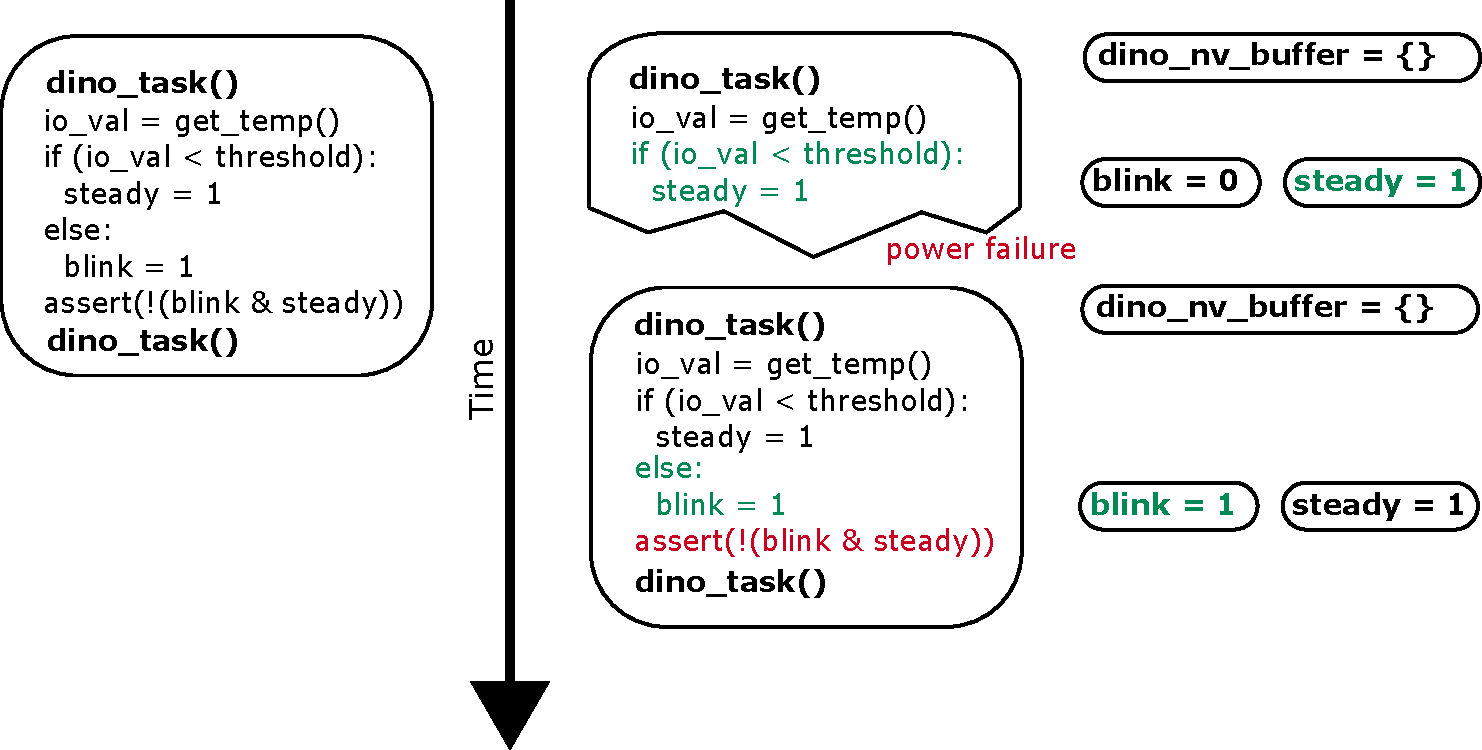
\includegraphics[width=1\columnwidth]{dino_io_violation.pdf}
\caption{Attempt to execute the code shown at left using the DINO runtime. The
state of the DINO buffer and the non-volatile variables, blink and steady are
shown to the right.}
\label{fig:dino}
\end{figure}

Any runtime system that relies strictly on WAR analysis to preserve idempotent
execution~\cite{dino, alpaca, ratchet} will experience the same failure mode
because the updates made along uncommitted branches will be allowed to persist.


\subsection{A discussion of non-idempotent behavior in intermittent programs}

In Figure \ref{fig:tax}, we present a flow chart of the taxonomy of
non-idempotent behaviors and their potentially buggy consequences.

\begin{figure}[ht]
\centering
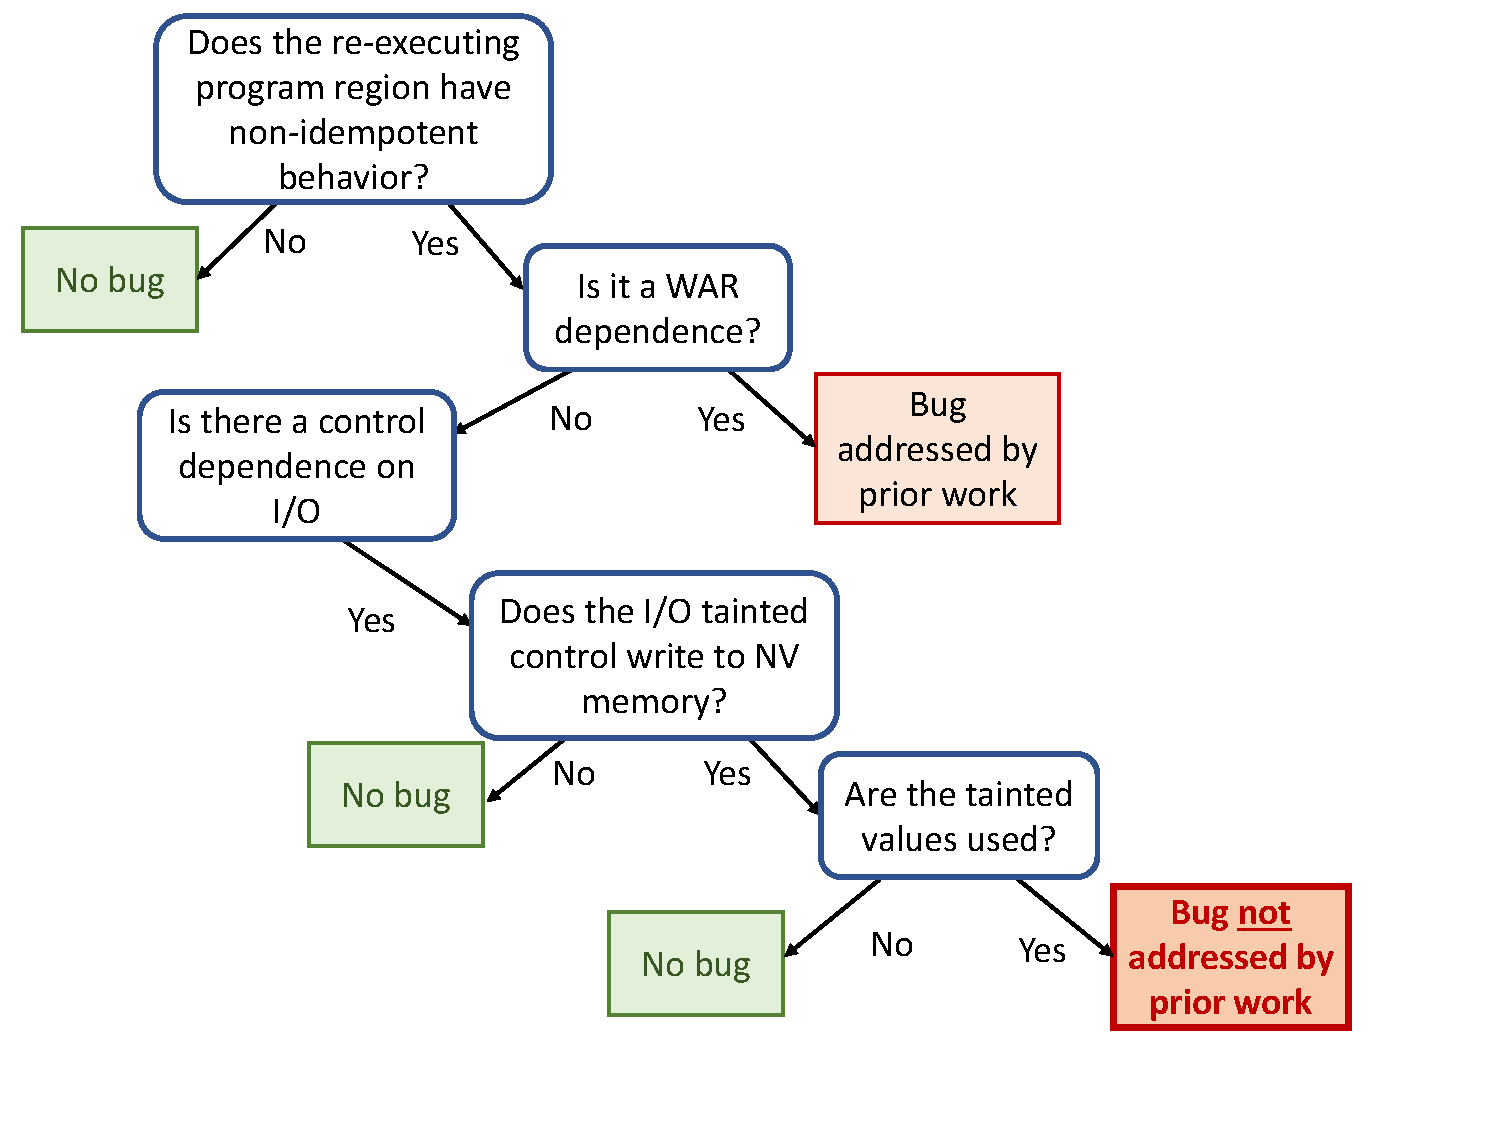
\includegraphics[width=1\columnwidth]{taxonomy.pdf}
\caption{Taxonomy of non-idempotent behavior and consequences}
\label{fig:tax}
\end{figure}
\paragraphb{Question 1: Does the program have non-idempotent behavior?}
Idempotent code can be re-executed arbitrarily without any changes to the
visible output~\cite{ratchet,dino}. Most new bugs introduced by computing under
intermittent power are due to memory inconsistencies caused by the unexpected
re-execution of code regions. If a program does not exhibit non-idempotent
behavior, it will not have any of the bugs we are studying.

\paragraphb{Questions 2 and 3: What is the cause of the non-idempotency?}
Non-idempotent behavior generally has two sources: write-after-read (anti)
dependencies and I/O operations.\footnote{Besides WAR dependencies and I/O,
there are some less common causes of non-idempotency, such as pointer-based
stack operations, as noted in prior work by Van Der Woude et al.
\cite{ratchet}.} Code re-execution after a WAR dependence creates direct
data-flow that did not exist in the original program, and I/O creates effects
that cannot be undone. Bugs off of WAR dependencies have been extensively
studied in prior work, and several runtime systems exist to fix them
\cite{ratchet, alpaca, dino}. While there could be other bugs
stemming from the use of irrevocable I/O operations, this paper specifically
explores memory inconsistencies stemming from branches that are control
dependent on non-idempotent input.

\paragraphb{Questions 4 and 5: When can an I/O dependent branch cause a bug?}
Not all I/O dependent branches necessarily lead to buggy behavior. To make
memory be in an inconsistent state, non-volatile variables must be written to on
at least one side of the branch, as they will still be visible to the program on
reboot. Furthermore, on a power fail and re-execution of the non-idempotent
region, such a tainted variable has to be the reaching definition for some use,
either in expected program execution or along the back-edge introduced by
re-executing. We discuss this further in Section [false positives]. If the
targets of the I/O dependent branch do write to non-volatile memory, however,
and there is some use of these tainted variables, this can cause bugs that have
not been addressed by prior work.
%		\item{Sometimes buggy behavior might only be exposed by re-orderings of
%		instructions during runtime. In such cases where the programmer %correctly
%		blocked the tainted variable from having any uses or wrote the exact same
%		non-volatile write set on both sides of the I/O branch, %compiler
%		optimizations might order the initializations on the wrong side of the reset
%		point [This would depend on the runtime system] or change %the order of the
%		non-volatile writes such that it is possible to write divergent sets on a
%		power fail. [Note: this needs to be written better.]} 

	

